Determine the best-fit hyperplane that predicts calories of a burger based upon the fat, carbohydrate, and protein content of the burger. Explicitly state the terms in the normal forms: $X$, $X^T  X$, $( X^T  X)^{-1}$, and $ X^T Y$.

\nnl \textbf{Solution: } Let the fat, carbs, and protein be the column vectors of $X$ and calories be the column vector of $Y$. Then
$$X = \begin{bmatrix}
    18 & 27 & 13\\
    11 & 25 & 13\\
    9 & 31 & 12\\
    17 & 38 & 20\\
    14 & 32 & 15\\
    16 & 32 & 15
\end{bmatrix} \wideand Y = \begin{bmatrix}
    310 \\ 250 \\ 250 \\ 390 \\ 320 \\ 330
\end{bmatrix}.$$
Then
$$X^T X = \begin{bmatrix}
    18 & 11 & 9 & 17 & 14 & 16\\
    27 & 25 & 31 & 38 & 32 & 32\\
    13 & 13 & 12 & 20 & 15 & 15
\end{bmatrix}
\begin{bmatrix}
    18 & 27 & 13\\
    11 & 25 & 13\\
    9 & 31 & 12\\
    17 & 38 & 20\\
    14 & 32 & 15\\
    16 & 32 & 15
\end{bmatrix}
=\begin{bmatrix}
    1267 & 2646 & 1275 \\
    2646 & 5807 & 2768 \\
    1275 & 2768 & 1332
\end{bmatrix}.$$
Expanding across the first row,
\begin{align*}
    \begin{vmatrix}
        1267 & 2646 & 1275 \\
        2646 & 5807 & 2768 \\
        1275 & 2768 & 1332
    \end{vmatrix} &= 1267 \begin{vmatrix}
        5807 & 2768 \\
        2768 & 1332
    \end{vmatrix} + 2646 \begin{vmatrix}
        2646 & 2768\\
        1275 & 1332
    \end{vmatrix} + 1275 \begin{vmatrix}
        2646 & 5807 \\
        1275 & 2768
    \end{vmatrix}\\
    &= 92617700 - (-12510288) -101741175\\
    &= 3386813.
\end{align*}
Since $\det (X^TX) \neq 0$ then the inverse exists.
$$\begin{bmatrix}
    X^TX \mid I_3
\end{bmatrix} = \begin{bmatrix}
    1267 & 2646 & 1275 &\bigm| & 1 & 0 & 0 \\
    2646 & 5807 & 2768 &\bigm| & 0 & 1 & 0 \\
    1275 & 2768 & 1332 &\bigm| & 0 & 0 & 1  
\end{bmatrix}$$
This row reduces to $\displaystyle \begin{bmatrix}
    I_3 \mid (X^TX)^{-1}
\end{bmatrix}$ in which
$$(X^TX)^{-1} = \over*{\num{3386813}} \begin{bmatrix}
    73100 & 4728 & -79797\\
    4728 & 62019 & -133406\\
    -79797 & -133406 & 356153
\end{bmatrix}.$$
Lastly, 
$$X^TY = \begin{bmatrix}
    18 & 11 & 9 & 17 & 14 & 16\\
    27 & 25 & 31 & 38 & 32 & 32\\
    13 & 13 & 12 & 20 & 15 & 15
\end{bmatrix} \begin{bmatrix}
    310 \\ 250 \\ 250 \\ 390 \\ 320 \\ 330
\end{bmatrix} = \vvec*{26970}{57990}{27830}.$$
Solving the normal equation, 
\begin{align*}
    \betah &= (X^TX)^{-1}X^TY\\
    &= \over*{\num{3386813}} \begin{bmatrix}
        73100 & 4728 & -79797\\
        4728 & 62019 & -133406\\
        -79797 & -133406 & 356153
    \end{bmatrix} \vvec*{26970}{57990}{27830}\\
    &= \over*{\num{3386813}} \vvec*{\num{24933210}}{\num{11306990}}{\num{23398960}}\\
    &\approx \vvec*{7.36185021}{3.3385339}{6.90884321}.
\end{align*}
Therefore the hyperplane of best fit is
$$\widehat{y} = 7.36185021 \cdot \text{(fat)} + 3.3385339 \cdot \text{(carbs)} + 6.90884321 \cdot \text{(protein)}.$$
Testing this on our data:
\notab{
    \begin{center}
        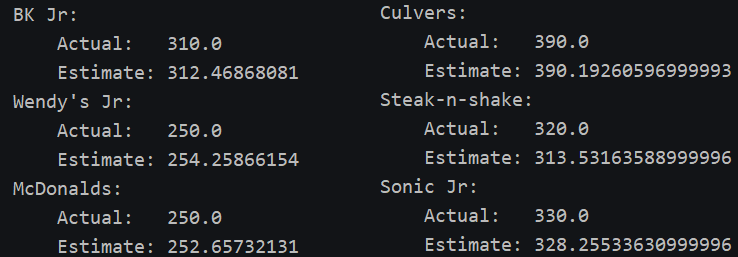
\includegraphics[height=2.25in]{estimate.png}
    \end{center}
}